% Created 2014-01-05 Sun 17:50
\documentclass[11pt]{article}
\usepackage[utf8]{inputenc}
\usepackage[T1]{fontenc}
\usepackage{fixltx2e}
\usepackage{graphicx}
\usepackage{longtable}
\usepackage{float}
\usepackage{wrapfig}
\usepackage{rotating}
\usepackage[normalem]{ulem}
\usepackage{amsmath}
\usepackage{textcomp}
\usepackage{marvosym}
\usepackage{wasysym}
\usepackage{amssymb}
\usepackage{hyperref}
\tolerance=1000
\author{Ted Wiles}
\date{\today}
\title{example2}
\hypersetup{
  pdfkeywords={},
  pdfsubject={},
  pdfcreator={Emacs 24.3.50.1 (Org mode 8.2.4)}}
\begin{document}

\maketitle
\tableofcontents

\section{An Example - a DCF Calculation.}
\label{sec-1}

\begin{table}[htb]
\caption{\label{DCF}DCF}
\begin{tabular}{rlrr}
Year & Growth Rate \footnotemark & Cash & Discounted Cash\\
\hline
0 & 0.03 & 500 & 500\\
1 & 0.15 \footnotemark & 575.00 & 527.52\\
2 & 0.15 \footnotemark[2]{} & 661.25 & 556.56\\
3 & 0.15 \footnotemark[2]{} & 760.44 & 587.20\\
4 & 0.15 \footnotemark[2]{} & 874.51 & 619.52\\
5 & 0.15 \footnotemark[2]{} & 1005.69 & 653.63\\
6 & 0.05 \footnotemark & 1055.97 & 629.64\\
7 & 0.05 \footnotemark[3]{} & 1108.77 & 606.54\\
8 & 0.05 \footnotemark[3]{} & 1164.21 & 584.28\\
9 & 0.05 \footnotemark[3]{} & 1222.42 & 562.84\\
10 & 0.05 \footnotemark[3]{} & 1283.54 & 542.18\\
10 & 0.03 & 22034.10 & 9307.44\\
 & 0.05 & 1 & 15677.35\\
\hline
COE= & 0.09 \footnotemark &  & \\
g= & 0.03 \footnotemark[1]{} &  & \\
\end{tabular}
\end{table}\footnotetext[1]{\texttt{\$g}}\footnotetext[2]{\texttt{\$g1t5}}\footnotetext[3]{\texttt{\$g6t10}}\footnotetext[4]{\texttt{\$COE}}

\begin{table}[htb]
\caption{\label{ScenarioManager}Scenario Manager}
\begin{tabular}{rr}
COE & DCF \footnotemark\\
\hline
.04 & 97480.87\\
.05 & 48332.71\\
.06 & 31973.63\\
.07 & 23810.54\\
.08 & 18924.93\\
.09 & 15677.35\\
.10 & 13365.25\\
.11 & 11637.39\\
.12 & 10298.65\\
\end{tabular}
\end{table}\footnotetext[5]{\texttt{`(org-table-xtras-eval-table "DCF" `(("COE" . \$1)) "DCF")}}
\section{Another Example - Simulating FOMC distributions}
\label{sec-2}

\begin{table}[htb]
\caption{\label{GDPProjections}Economic Projections of FOMC Members, September 2013}
\begin{tabular}{rrrrr}
Year & CT-Lower \footnotemark \textsuperscript{,}\,\footnotemark & CT-Upper \footnotemark[6]{} & Range-Lower \footnotemark[6]{} \textsuperscript{,}\,\footnotemark & Range-Upper \footnotemark[6]{} \textsuperscript{,}\,\footnotemark[8]{}\\
\hline
2013 & 2.2 & 2.3 & 2.2 & 2.4\\
2014 & 2.8 & 3.2 & 2.2 & 3.3\\
2015 & 3.0 & 3.4 & 2.2 & 3.6\\
2016 & 2.5 & 3.2 & 2.1 & 3.5\\
Long Run & 2.2 & 2.4 & 1.8 & 2.5\\
\end{tabular}
\end{table}\footnotetext[6]{\url{http://www.federalreserve.gov/monetarypolicy/files/fomcprojtabl20131218.pdf}}\footnotetext[7]{The central tendency excludes the three highest and three lowest projections for each variable in each year.}\footnotetext[8]{The range for a variable in a given year includes all participants’ projections, from lowest to highest, for that variable in that year.}

I want to try and draw from this distribution of FOMC participants.

First, let's assume that the projections are uniform within each CLT range (e.g. the projections occur uniformly between 2.8 and 3.2 in 2014).

There are three more observations occuring somewhere between the lower range bound and the lower central tendency bound, three more observations occuring somewhere between the upper range bound and the upper central tendency bound, and there are 19 observations in total.

So, we can assume that each true value has a 3/19 chance of landing in the lower region, 3/19 chance of landing in the upper region, and 13/19 change of landing in the middle region, and, a uniform distribution within each of these regions:

\begin{tabular}{ll}
Year & 2013\\
\hline
CT-Lower & 2.20 \footnotemark\\
CT-Higher & 2.30 \footnotemark\\
Range-Lower & 2.20 \footnotemark\\
Range-Upper & 2.40 \footnotemark\\
\hline
Seed 1 & 0.82 \footnotemark\\
Seed 2 & 0.64 \footnotemark[13]{}\\
Simulated Draw & 2.364 \footnotemark\\
\end{tabular}\footnotetext[9]{\texttt{\$CTLOW}}\footnotetext[10]{\texttt{\$CTHIGH}}\footnotetext[11]{\texttt{\$RANGELOW}}\footnotetext[12]{\texttt{\$RANGEHIGH}}\footnotetext[13]{\texttt{random(1.0)}}\footnotetext[14]{\texttt{`(tw-distribution @-2 @-1 "\$RANGELOW" "\$RANGEHIGH" "\$CTLOW" "\$CTHIGH")}}

\subsection{Simulated Distribution}
\label{sec-2-1}

Figure \ref{fig:Sim} shows the results of drawing a 60-observation sample from these distributions gives the following cumulative density plots 

\begin{figure}[htb]
\centering
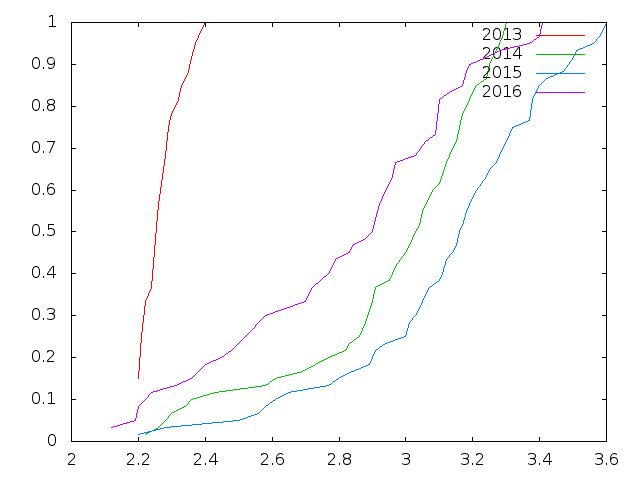
\includegraphics[width=.9\linewidth]{./example2.png}
\caption{\label{fig:Sim}Simulated Distribution of FOMC predictions.}
\end{figure}
\section{Appendix: Lisp code}
\label{sec-3}

There are three lisp code functions I used in this org-mode file. The first, \texttt{tw-distribution} draws the FOMC distribution as the combination of three uniform distrubions. GDP-ref gets remote ranges from the \texttt{GDPProjections} table. I coded it in lisp to save space in the TBLFM line. Similarly, \texttt{eval-table-list} evaluates the simulation spreadsheets with some given arguments. I had to write this function in order to perform the \texttt{gdp-ref} lookup before \texttt{org-table-xtras-eval-table} was evaluated.

\begin{verbatim}
(defun tw-distribution (r1 r2 rangelow rangehigh ctlow cthigh)
  (let ((rangehigh (string-to-int rangehigh))
	(rangelow (string-to-int rangelow))
	(ctlow (string-to-int ctlow))
	(cthigh (string-to-int cthigh))
	(r1 (string-to-int r1))
	(r2 (string-to-int r2)))
  (cond ((> r1 (/ 16 19)) (+ cthigh (* r2 (- rangehigh cthigh))))
	((< r1 (/ 3 19))  (+ rangelow (* r2 (- ctlow rangelow))))
	(t (+ ctlow (* r2 (- cthigh ctlow)))))))

(defun gdp-ref (val col)
  (org-lookup-first 
    val
    (org-table-get-remote-range "GDPProjections" "@2$1..@>$1")
    (org-table-get-remote-range "GDPProjections" (concat  "@2$" col "..@>$" col))))

(defun eval-table-list (year)
  (let ((arglist (list (cons "year" year)
		       (cons "CTLOW" (gdp-ref year "2"))
		       (cons "CTHIGH" (gdp-ref year "3"))
		       (cons "RANGELOW" (gdp-ref year "4"))
		       (cons "RANGEHIGH" (gdp-ref year "5")))))
    (princ arglist)
    (org-table-xtras-eval-table "Sample" arglist "Sim")))
\end{verbatim}
% Emacs 24.3.50.1 (Org mode 8.2.4)
\end{document}
